\section{Home}
Pemrograman python adalah bahasa pemrograman terpopuler di tahun 2016 menurut tiobe. Python juga memiliki sintak atau aturan penulisan code pemrograman. Salah satu bagian Home merupakan halaman pengantar untuk mempelajari python . sebelum ketahapan yang baru selain home ini pembaca memerlukan pengertian yang lain yaitu seperti enverinmoment setup, syntax dan lain lain, awal untuk penulis jelakan yaitu pengertian tentang class pada python untuk mengantarkan logika dan pengetahuan apa itu class.
Bahasa Pemrograman Python sudah dirasakan cukup matang untuk memecahkan masalah dalam dunia komputasi dan pengembangan sistem informasi. Manajemen paket Red Hat Linux, Blender,  PyGame, ZOPE (Framework Python untuk web services) telah membuktikan kepada kita semua bahwa Python merupakan bahasa pemrograman yang perlu diajarkan pada perguruan tinggi, terutama konsep interpreter, object oriented programming dan lainnya.
Phyton dapat berjalan dibanyak platform atau sistem operasi seperti windows, linux/unix, mac OS X, OS/2, amiga, palm handhelds dan telepon genggam nokia. namun saat ini python juga sudah masuk kedalam virtual java dan NET. Python memiliki beberapa keunggulan, yaitu :
\begin{enumerate}
\item Syntaxnya sangat bersih dan mudah dibaca
\item Kemampuan melakukan pengekan syntaxnya yang kuat
\item Berorientasi objek secara intuisif
\item Kode-kode prosedure dinyatakan pada ekspresi natural
\item Modularitas yang penuh, mendukung hirarki paket
\item Penanganan error dilakukan berdasar pada eksepsi
\item Tipe-tipe data dinamis berada pada tingkat sangat tinggi
\item Library standar dapat diperluas dan modul dari pihak ketiga dapat dibuat secara virtual untuk setiap kebutuhan
\item Ekstensi dan modul-modul dapat secara mudah ditulis dalam C, C+ (atau java untuk Jython atau NET untuk IronPytho)
\item Dapat dimasukan kedalam aplikasi sebagai antar muka skrip
\end{enumerate}


\subsection{Kenapa alasan memilih Pemograman Phyton}
\begin{enumerate}
\item Python memiliki konsep desain yang bagus dan sederhana, yang berfokus pada kemudahan dalam penggunaan. Kode Python dirancang untuk mudah dibaca, dipelajari, digunakan ulang, dan dirawat. Selain itu, Python juga mendukung pemograman berorientasi objek dan pemograman fungsional.
\item Python dapat meningkatkan produktivias dan menghemat waktu bagi para programmer.Untuk memperoleh hasil program yang sama, kode Python juga jauh lebih sedikit dibandngkan dengan kode yang ditulis menggunakan bahasa-bahasa pemograman lain seperti C, C++,C\# maupun Java. Coba lihat ilustrasi gambar dibawah ini:Bagaimana menurut kamu ? Sudah pasti Pyhton lebih sederhana dibanding bahasa-bahasa pemograman lain.
\item Program yang ditulis menggunakan Python ,dapat dijalankan di hampir semua sistem operasi (Unix, Windows, Mac OS X, dll), termasuk untuk perangkat-perangkat mobile.
\item Python memiliki banyak dukungan pustaka yang dikembangakan oleh pihak ketiga, misalnya pustaka untuk pengembangan web, pengembangan aplikasi visual (berbasis GUI), pengembangan permainan komputer (game), dan masih banyak lagi yang lainnya.
\item Melalui mekanisme tertenu, kode Python dapat diintegrasikan dengan aplikasi yang ditulis dalam bahasa pemograman lain. Sebagai contoh, kode Python dapat dipanggil dari kode C/C++, dan begitu juga perkembangan .NET Framework.
\item Terakhir, Python bersifat gratis atau bebas (free) dan open source, meskipun digunakan untuk kepentingan komersial.
\end{enumerate}

\subsection{Ranah Aplikasi Python}
Python dapat digunakan untuk membangun aplikasi-aplikasi berjalan pada banyak fungsi. diantaranya adalah sebagai berikut :
\begin{enumerate}
\item Pengembangan web dan internet. Dimana python mampu mengembangkan web dan internet seperti : penulisan skrip Common Gateway Internet (CGI), pengembangan frameworks seperti djago dan turbo gears, python juga mendukung penuh HTML, dan XML, pemrosesan e-mail, pemrosesan RRS feeds dll.
\item Akses terhadap database. antar muka open database connectivity (ODBC) untuk MySQL, Oracle,postgreSQL, SybaseODBC. dan juga mampu menyediakan Appication Programming Interface (API)
\item Pengembangan Graphical User Interface (GUI) pada Dekstop
\item Keperluan perhitung scientific dan numeris.
\item Pengembangan perangkat lunak komputer.
\item Pengembangan jaringan komputer.
\end{enumerate}

\subsection{interpreter python}
Bahasa pemrograman pyhton dilengkapi dengan suatu fasilitas seperti shell di linux, yang digunakan secara berulang dikemudian hari. untuk keperluan pernulisan ekspresi kompleks, kita dapat membuatnya dalam sebuah script yang dibantu dengan adanya teks editor. berikut adalah contoh dari statement dasar, perulangan dan seleksi
 
\subsection{Komputasi}
komputasi dengan bahasa: Statistik Sederhana
mari kita kembali ke eksplorasi kita tentang cara membawa sumber daya komputasi kita untuk menghasilkan teks dalam jumlah banyak.
Pada bagian ini, kita mengambil pertanyaan tentang apa yang membuat teks menjadi distinc, dan gunakan metode otomatis untuk menemukan kata-kata dan ekspresi teks yang khas.
Sebelum melanjutkan lebih lanjut, Anda mungkin ingin memeriksa pemahaman Anda tentang bagian terakhir dengan memprediksikan output dari kode berikut. Anda bisa menggunakan penerjemah untuk memeriksa apakah Anda benar. Jika Anda tidak yakin bagaimana melakukan tugas ini, sebaiknya Anda meninjau bagian sebelumnya sebelum melanjutkan lebih jauh.

\subsection{fitur dan keunggulan python}
Beberapa fitur yang dapat dikatakan sebagai keunggulan python yaitu :
\begin{enumerate}
\item Python is powerful and fast, artinya python merupakan suatu kumpulan modul-modul yang sangat baik  dan dapat menangani secara praktis setiap domain masalah.
\item Python plays well with others, artinya python dapat beritegrasi dengan Component Object Model (COM), NET dan objek-objek Common Object Request Broker Architecture (COBRA).
\item Python runs everywhere, artinya python tersedia untuk berbagai macam sistem operasi seperti windows, unix atau linux, OS/2, mac, Amiga dll.
\item Python is friendly and easy to learn, artinya python sangat bersahabat bagi penggunanya.
\item Python is open, artinya python dibawah lisensi open source yang membuatnya dapat disebarkan secara bebas nbahkan untuk keperluan komersil.
\end{enumerate}

\subsection{Script Python}
    Seringkali pengguna harus menuliskan ekspresi yang cukup kompleks dan akan digunakan secara berulang di kemudian hari. Untuk keperluan penulisan ekspresi kompleks, kita dapat membuatnya dalam sebuah script yang dibantu dengan adanya teks editor. Penulis menggunakan vi teks editor default yang terdapat pada distro GNU/Linux.

\subsection{Kelebihan dan Kekurangan}
\subsubsection{Kelebihan}
\begin{enumerate}
\item Tidak ada tahapan kompilasi dan penyambungan (link) sehingga kecepatan perubahan pada masa pembuatan sistem aplikasi meningkat.
\item Tidak ada deklarasi tipe data yang merumitkan sehingga program menjadi lebih sederhana, singkat, dan fleksible.
\item Manajemen memori otomatis yaitu kumpulan sampah memori sehingga dapat menghindari pencacatan kode.
\item Tipe data dan operasi tingkat tinggi yaitu kecepatan pembuatan sistem aplikasi menggunakan tipe objek yang telah ada.
\item Pemrograman berorientasi objek.
\item Pelekatan dan perluasan dalam C.
\item Terdapat kelas, modul, eksepsi sehingga terdapat dukungan pemrograman skala besar secara modular.
\item Pemuatan dinamis modul C sehingga ekstensi menjadi sederhana dan berkas biner yang kecil.
\item Pemuatan kembali secara dinamis modul phyton seperti memodifikasi aplikasi tanpa menghentikannya.



\begin{figure}[ht]
	\centerline{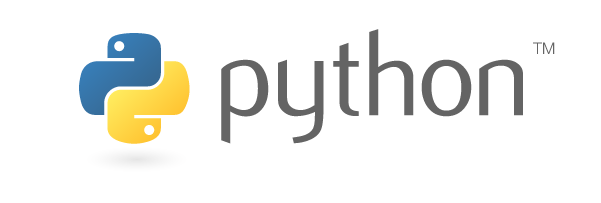
\includegraphics[width=0.70\textwidth]{figures/python}}
	\caption{Logo}
	\label{Logo}
\end{figure}

\section{python}
Pemrograman python adalah bahasa pemrograman terpopuler di tahun 2016 menurut tiobe. Python juga memiliki sintaks atau aturan penulisan \textit{code} pemrograman. Salah satu bagian Home merupakan halaman pengantar untuk mempelajari python. Sebelum ketahapan yang baru selain home ini pembaca memerlukan pengertian yang lain yaitu seperti enverinmoment setup, syntax dan lain lain, awal untuk penulis jelakan yaitu pengertian tentang \textit{class} pada python untuk mengantarkan logika dan pengetahuan apa itu \textit{class}.

Class itu merupakan class yang didalam nya mempunyai metode yang sesuai dengan fungsinya, contoh di kehidupan nyata seperti kelas belajar sebagai class nya da isi dari kelas itu seperti bangku, sepidol, dan lain lain itu merupakan metode dari class dan metode itu berfungsi seperti fungsi itu sendiri seperti spidol untuk menulis itu contoh nya di sesuaikan dengan fungsi.
\subsection{Pembuatan class pada python}
Kita awali dengan sebuah kata kunci. Yaitu  ``class`` yang kemudian di ikuti dengan  ``nama class nya`` terkahir membuat kurung buka dan tutup serta membuat tanda titik dua  ``()`` dan ``:``kalo synax nya seperti ini.

namaClass()

untuk memanggil metode kita cukup menggunakan memanggil class yang kemudian di ikuti dengan pemanggilan nama metode yang tersedia di dalam class tersebut dengan di pisahkan oleh tanda titik seperti 
\begin{verbatim}
namaClass().namaMetode()
\end{verbatim}
ingin lebih mudah kita tampung classnya dulu ke variable 

penampung = namaClass() 
\begin{verbatim}
penampung.namaMetode()
\end{verbatim}
di dalam sebuah class yang dibuat biasanya terdapat init itu disediakan langsung oleh python nya jadi seperti ini 


\begin{verbatim}

 class namaClass():
def init (self,parameter):
itu code program yang pertama kali kalian buat
def metode 1 (self,parameter):
isi metode
def metode 2 (self):
 isi metode
 
 \end{verbatim}
 
Setelah menjelaskan class kita akan menjelaskan variable seperti tadi penampung class, nah variable bisa di artikan sebagai huruf atau kata tujuan nya untuk mempermudah proses penulisan sebuah program. Contoh dalam kehidupan nyata seperti gelas atau ember, ambil contoh ember kita ketahui bahwa ember bisa di isi dengan air, pasir, tanah dan lain lain, nah ember itu sebagai variable da nisi variable nya itu adalah air, tanah, pasir dan lain lain. 
Contoh variable seperti ini

\begin{verbatim}
 Variable=  "ini string atau teks"
\end{verbatim}

\begin{verbatim}
Print( "nilai isi dari variable1 adalah: ",variable1)
Print( "nilai atau isi dari variable2 adalah:",variable2)
\end{verbatim}

Ada beberapa hal yang harus di ketahui seperti input, data operation danlain lain seperti ini

\begin{itemize}
	\item input 
	\item data
	\item opration
	\item output
	\item condutional
	\item looping
	\item subroutine
\end{itemize}

Tahapan ini merupakan proses memasukan data ke dalam proses komputer melalui peralatan input. Pada bahasa Python, untuk menerima masukan dari pengguna yaitu dengan menggunakan method input() dan raw $_$input(). 
Data adalah bahan mentah yang akan diolah menjadi informasi sehingga dapat berguna dan dimanfaatkan oleh pengguna. Data dapat berupa variabel, konstanta, atau yang berisi bilangan, kalimat, dan lainnya. Tipe data berupa string, number, list, tuple, dan lainnya.  \subsection {Operation}

Operation adalah yang akan mengubah suatu nilai menjadi nilai lain. Yang termasuk operation atau yang biasa disebut dengan operator adalah operator aritmatika, operator assignment, dan lainnya. 
\subsection {Output}

Output adalah menuliskan informasi yang ditampilkan dilayar, disk, atau ke salah satu unit I/O. Pada Python 2.0, untuk menampilkan output dengan menulis sintax print. Sedangkan pada Python 3.0 dengan menggunakan fungsi print().

\subsection {Conditional}
Merupakan jumlah perintah yang akan dijalankan jika kondisi tertentu sudah terpenuhi. Jika username dan password yang dimasukan benar, maka akan menampilkan halaman utama. Hal ini bisa disebut conditional. Pada conditional, Python menggunakan pernyataan if, else, dan elif. 
\subsection {Looping}
Perintah yang akan berjalan beberapa kali, selama kondisi yang ditentukan atau kondisi yang terpenuhi. Pada looping ini, Python menggunakan pernyataan for dan while untuk melakukan perulangan. 
\subsection {Subroutine}
Perintah yang bisa dijalankan dengan cara memanggil namanya. Sering disebut sebagai functionatau method. Pada bahasa pemrograman Python, untuk menggunakan function atau method yaitu dengan menggunakan pernyatan def nama _ $function(). 
Fungsi def dalam python
Penggunaan fungsi tanpa parameter
Command=fungsi() 
Deklarasi command= def fungsi() 
Pemanggilan fungsi, parameter sesuai dengan kata kunci seperti tadi class
Command= fungsi(arg=1, arg2=2)
Deklarasi command – def fungsi (arg2,arg2)
Pemanggilan fungsi, parameter sesuai dengan posisi 
Command= fungsi() 
Deklarasi command – def fungsi (x)  Pemanggilan fungsi parameter sesuai dengan argument posisional tuple
Command= fungsi((1,2).(1,3)) 
Deklarasi command – def fungsi (*args)
Pemanggilan fungsi, parameters ssesuai argument kata kunci dictionary 
Command= fungsi (bahasa= ‘python’,versi=’2.2’)
Deklarasi command = def fungsi (**args)
Itu adalah cara memanggil dalam code python pemrograman jadi ada nenerapa fungsi yang dibutuhkan penulisan dengan tepat maka sebab itu dengan sebab itu buaat lah penulisan yang mudah. Karena pemrograma python sangan sensitive bila ada kesalahan sedikit di penulisan atau symbol yang tertinggal. 

\subsection {Sejarah}
Bahasa pemrograman Python adalah bahasa yang dibuat oleh seorang keturunan Belanda yaitu Guido van Rossum. Awalnya, pembuatan bahasa pemrograman ini adalah untuk membuat skrip bahasa tingkat tinggi pada sebuah sistem operasi yang terdistribusi Amoeba. Python telah digunakan oleh beberapa pengembang dan bahkan digunakan oleh beberapa perusahaan untuk pembuatan perangkat lunak komersial. Pemrograman bahasa python ini adalah pemrogram gratis atau freeware, sehingga dapat dikembangkan, dan tidak ada batasan dalam penyalinannya dan mendistribusikan. 
\subsection{Dukungan Komunitas yang Aktif}
Python adalah salah satu pemrograman yang terus berkembang dan bertahan dikarenakan dukungan komunitas yang aktif diseluruh dunia. Banyak forum-forum ataupun blogger-blogger yang sering membagi pengalaman dalam menggunakan python. Hal ini memudahkan bagi pengguna pemula maupun pengembang untuk bertanya dan sharing tentang ilmu pemrograman ini. 
\subsection{Kelebihan dan Kekurangan}
Kelebihan :
\begin{enumerate}
\item Tidak ada tahapan kompilasi dan penyambungan (link) sehingga kecepatan perubahan pada masa pembuatan sistem aplikasi meningkat. 
\item Tidak ada deklarasi tipe data yang merumitkan sehingga program menjadi lebih sederhana, singkat, dan fleksible.
\item Manajemen memori otomatis yaitu kumpulan sampah memori sehingga dapat menghindari pencacatan kode.
\item Tipe data dan operasi tingkat tinggi yaitu kecepatan pembuatan sistem aplikasi menggunakan tipe objek yang telah ada.
\item Pemrograman berorientasi objek. 
\item Pelekatan dan perluasan dalam C.
\item Terdapat kelas, modul, eksepsi sehingga terdapat dukungan pemrograman skala besar secara modular.
\item Pemuatan dinamis modul C sehingga ekstensi menjadi sederhana dan berkas biner yang kecil 
\item Pemuatan kembali secara dinamis modul phyton seperti memodifikasi aplikasi tanpa menghentikannya. 
\item Model objek universal kelas Satu.
\item Konstruksi pada saat aplikasi berjalan.
\item Interaktif, dinamis dan alamiah.
\item Akses hingga informasi interpreter.

\item Portabilitas secara luas seperti pemrograman antar platform tanpa ports
\item Kompilasi untuk portable kode byte sehingga kecepatan eksekusi bertambah dan melindungi kode sumber. 
\item Antarmuka terpasang untuk pelayanan keluar seperti perangkat Bantu system, GUI, persistence, database, dll.
\end{enumerate}
Kekurangan:
\begin{enumerate}
\item Beberapa penugasan terdapat diluar dari jangkauan python, seperti bahasa pemrograman dinamis lainnya, python tidak secepat atau efisien sebagai statis, tidak seperti bahasa pemrograman kompilasi seperti bahasa C. 

\item Disebabkan python merupakan interpreter, python bukan merupakan perangkat bantu terbaik untuk pengantar komponen performa kritis.
\item Python tidak dapat digunakan sebagai dasar bahasa pemrograman implementasi untuk beberapa komponen, tetapi dapat bekerja dengan baik sebagai bagian depan skrip antarmuka untuk mereka.
\item Python memberikan efisiensi dan fleksibilitas tradeoff by dengan tidak memberikannya secara menyeluruh. Python menyediakan bahasa pemrograman optimasi untuk kegunaan, bersama dengan perangkat bantu yang dibutuhkan untuk diintegrasikan dengan bahasa pemrograman lainnya.
\item Banyak terdapat referensi lama terutama dari pencarian google, python adalah pemrograman yang sangat lambat. Namun belum lama ini ditemukan bahwa Google, Youtube, DropBox dan beberapa software sistem banyak menggunakan Python.

\item Kini Python menjadi salah satu bahasa pemrograman yang populer digunakan oleh pengembangan web, aplikasi web, aplikasi perkantoran, simulasi, dan masih banyak lagi. Hal ini disebabkan karena Python bahasa pemrograman yang dinamis dan mudah dipahami.
\item Selain itu, sekarang telah tersedia berbagai situs kursus yang bagus untuk mempelajari bahasa pemrograman Python ini sehingga pembaca maupun developer pemula yang akan mempelajari bahasa ini akan menjadi lebih mudah karena dapat berlatih dimanapun dan kapanpun selama terhubung dengan Internet.
\item Menariknya, berbagai situs kursus gratis ini menawarkan metode pembelajaran yang interaktif sehingga mudah dimengerti oleh pesertanya.
\end{enumerate}
Python merupakan pemograman yang tidak pernah di compile secara full. Jika kamu sudah menyelesaikan programnya dan kamu ingin mengirim ke teman atau di bagikan ke internet maka teman atau orang lain dapat mengubah kode di program kamu karena program di buka di notepad, python akan tetap berbentuk kode yang sama tidak acak acakan sehingga orang lain dapat memahami pemograman yang kamu buat.

$>$$>$$>$ Python 2.4.3 ( $  \#  $1, Nov 11 2010, 13:34:43) [GCC 4.1.2 20080704 (Red Hat 4.1.2-48)] on linux2 Type "help", "copyright", "credits" or "license" for more information.

Ketik teks berikut pada prompt Python dan tekan Enter:

print ``Hello, Python!``


Jika Anda menjalankan versi baru Python, Anda perlu menggunakan pernyataan cetak dengan tanda kurung seperti pada cetak (``Halo, Python!``) . Namun dengan versi Python 2.4.3, ini menghasilkan hasil sebagai berikut: 

Hello, Pyhton!


\subsection{Elemen Dasar Python}
Bahasa pemrograman python memiliki beberapa elemen penting, diantaranya yaitu :
\begin{enumerate}
	\item Himpunan Karakter
		Semua karakter di python terdiri dari huruf besar, huruf kecil, angka dan simbol-simbol lainnya yang terdapat pada keyword dapat digunakan untuk menandai atau memberikan nama terhadap sebuah data atau object.
	\item Pengenal 
		Pengenal (identifier) merupakan suatu nama yang biasa dipakai oleh user (programmer) untuk menamakan : variabel, konstanta, tipe data, fungsi, label, objek, serta hal-hal lain. Karena python memiliki penamaan case sensitive maksudnya huruf besar dan kecil berbeda.Contoh : No\_mahasiswa berbeda dengan no\_mahasiswa
	\item Nama Variabel harus diawali dengan huruf atau karakter garis bawah, selanjutnya dapat diikuti dengan huruf maupun angka atau tanda garis bawah.Nama Variabel tidak boleh diawali dengan angka.
	\item Nama Variabel tidak boleh menggunakan operator-operator aritmatika dan karakter khusus.
	\item jika nama variabel terdiri dari dua atau lebih, maka antar kata tidak diperbolehkan menggunakan spasi
	\item Nama Variabel tidak boleh menggunakan kata-kata yang telah memiliki arti khusus dalam bahasa python.
	\item Penggunaan huruf kecil dan huruf besar dibedakan.
	\item Panjang maksimal suatu variabel adalah 32 karakter sehingga jika mendeklarasikan suatu variabel yang panjangnya lebih dari 32 karakter, secara otomatis sistem tetap akan mengenali sepanjang 32 karakter saja.
	\item Kata Kunci
\end{enumerate}
		Kata kunci (keywords) merupakan pengenal ke sistem python yang mempunyai arti khusus bagi interpreter python dan kata kunci juga merupakan kumpulan kata yang dicadangkan. kata-kata ini tidak boleh digunakan sebagai identifier.


\subsection{Pemrograman Mode Script}
Memohon interpreter dengan parameter script memulai eksekusi script dan berlanjut sampai script selesai. Saat skrip selesai, juru bahasa tidak lagi aktif. Mari kita tuliskan program Python sederhana dalam sebuah naskah. File Python memiliki ekstensi .py. Ketik kode sumber berikut di file.
Objek Dengan Python, seperti semua bahasa berorientasi objek, ada kumpulan kode dan data yang disebut objek, yang biasanya mewakili potongan dalam model konseptual suatu sistem. Objek dengan Python dibuat (yaitu, instantiated) dari template yang disebut kelas (yang akan dibahas kemudian, sebanyak bahasa dapat digunakan tanpa memahami kelas). Mereka memiliki atribut, yang mewakili berbagai potongan kode dan data yang membentuk objek. Untuk mengakses atribut, seseorang menuliskan nama objek yang diikuti oleh suatu periode (selanjutnya disebut titik), diikuti dengan nama atribut. 
Contohnya adalah atribut 'atas' dari string, yang mengacu pada kode yang mengembalikan salinan string di mana semua huruf adalah huruf besar. Untuk mendapatkan ini, perlu untuk memiliki cara untuk merujuk ke objek (dalam contoh berikut, jalan adalah string literal yang membangun objek). 
Paradigma : Multi-paradigm: object-oriented, imperative, functional, procedural, reflective
Muncul Tahun : 1991
Perancang : Guido van Rossum
Pengembang : Python Software Foundation
Rilis terbaru : 3.2.3 / 11 April 2012; 46 hari lalu 2.7.3 / 11 April 2012; 46 hari lalu /
Sistem pengetikan: duck, dynamic, strong
Implementasi : CPython, IronPython, Jython, Python for S60, PyPy
Dialek : Cython, RPython, Stackless Python
Terpengaruh oleh : ABC,ALGOL 68,C,C++,Dylan Haskell,Icon,Java,Lisp,Modula-3,Perl
Mempengaruhi : Boo, Cobra, D, Falcon, Groovy, JavaScript, Ruby
Sistem operasi : Cross-platform
Lisensi : Python Software Foundation License,GNU GPL
Situs web : python.org

